\chapter{Complete examples of \PD Maps}

The following maps present complete examples of SBGN Process Descriptions representing biological processes. They by no means exhaust the possibilities of  \SBGNPDLone.

\fig{glycolysis} presents an example of metabolic pathway, that exemplifies the use of the \glyph{EPNs} \glyph{simple chemical} and \glyph{macromolecule}, \glyph{clone marker}, the \glyph{PN} \glyph{process}, and the \glyph{connecting arcs} \glyph{consumption}, \glyph{production} and \glyph{catalysis}.

\begin{figure}[htb]
\begin{center}
\scalebox{0.4}{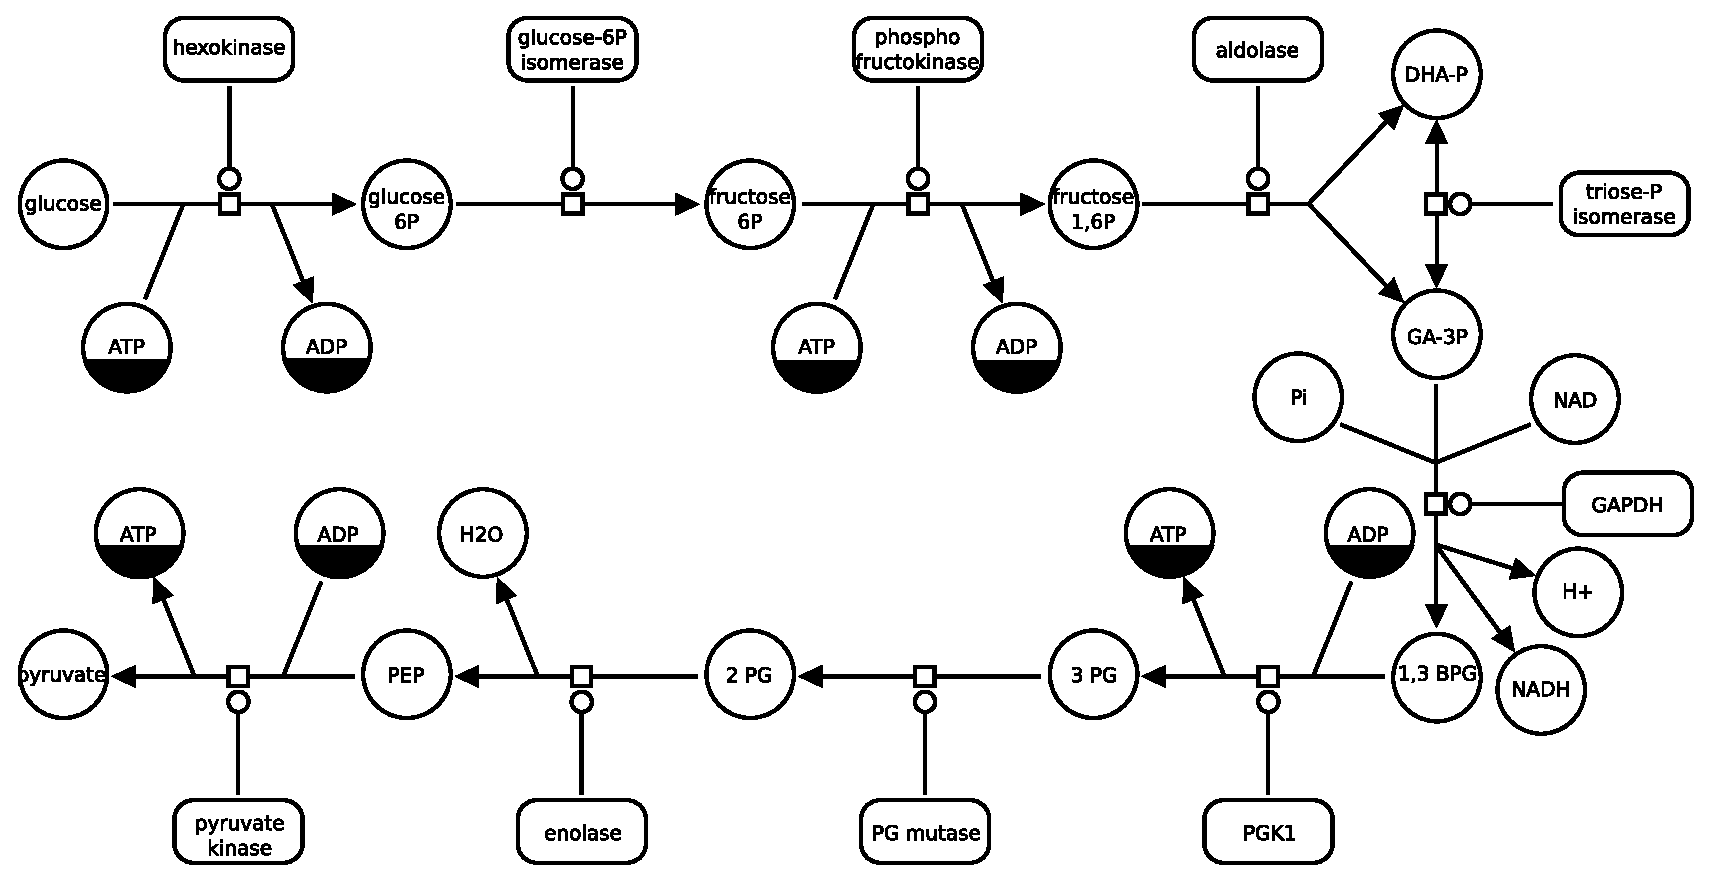
\includegraphics{examples/glycolysis}}
\caption{Glycolysis. This example illustrates how SBGN can be used to describe metabolic pathways.}\label{fig:glycolysis}
\end{center}
\end{figure}

\fig{insulin} presents an example of signalling pathway, that exemplifies in addition the use of the \glyph{EPN} \glyph{complex}, the \glyph{state variable}, the \glyph{container} \glyph{compartment}, the \glyph{submap}, the \glyph{PNs} \glyph{association} and \glyph{phenotype}, and the \glyph{connecting arc} \glyph{stimulation}. Note the complex IGF and IGF receptor, located on the boundary of the compartment. This position is only for user convenience. The complex has to belong to a given compartment in \SBGNPDLone.

\begin{figure}[htb]
\begin{center}
\scalebox{0.4}{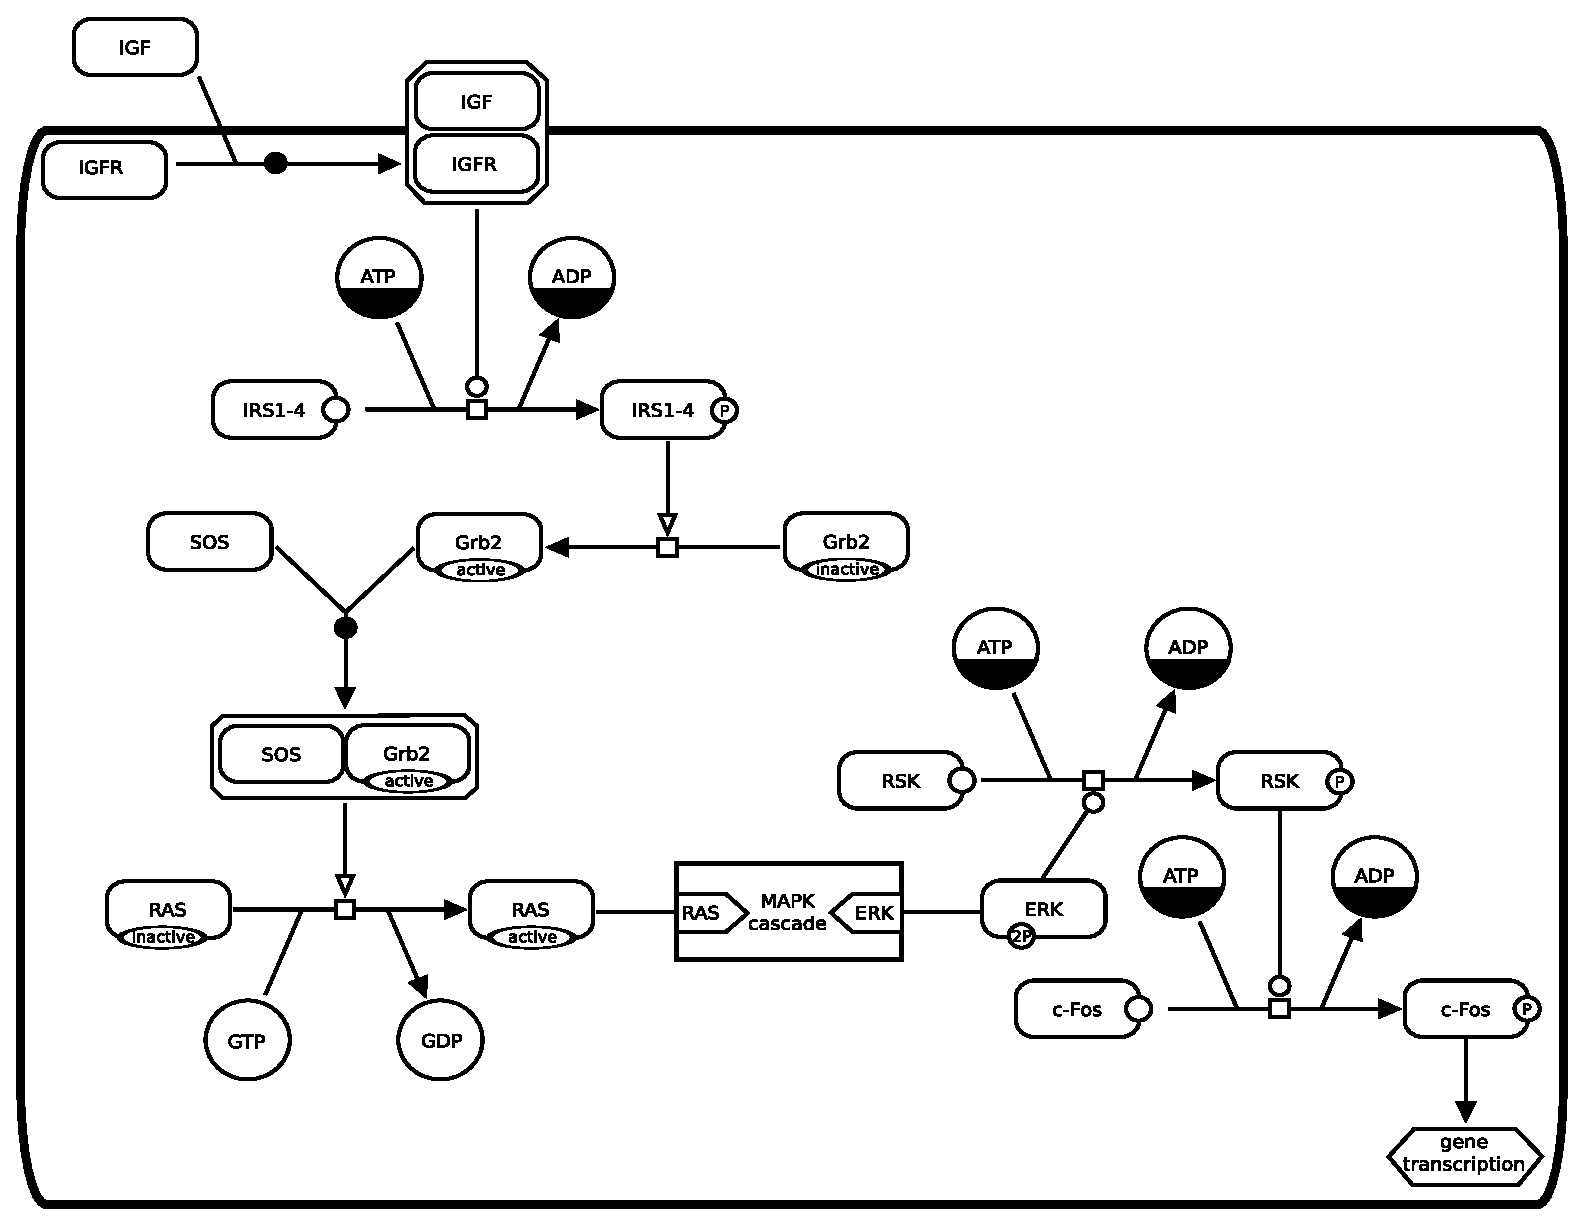
\includegraphics{examples/insulin}}
\caption{Insulin-like Growth Factor (IGF) signalling. This example shows the use of compartments and how details can be hidden by using a submap. The submap is shown on \fig{mapk}.}\label{fig:insulin}
\end{center}
\end{figure}

\fig{mapk} is an expanded version of the submap present on the map present in \fig{insulin}. It shows the use of \glyph{tag}.

\begin{figure}[htb]
\begin{center}
\scalebox{0.3}{\includegraphics{examples/MAPK}}
\caption{The expanded submap of the previous map showing the MAPK cascade.}\label{fig:mapk}
\end{center}
\end{figure}

\fig{muscle} introduces an SBGN \PD that spans several compartments. Note that the compartment ``synaptic vesicle'' is not \textbf{contained} in the compartment ``synaptic button'' but \textbf{overlaps} it. The \glyph{simple chemical} ``ACh'' of the ''synaptic vesicle`` is not the same \glyph{EPN} than the ``ACh'' of the ``synaptic button'' and of ``synaptic cleft''.  The situation is similar with the compartments ``ER'' and ``muscle cytosol''.  The map exemplifies the use of the \glyph{PNs} \glyph{omitted} and \glyph{dissociation}, and the \glyph{connecting arc} \glyph{necessary stimulation}.

\begin{figure}[htb]
\begin{center}
\scalebox{0.5}{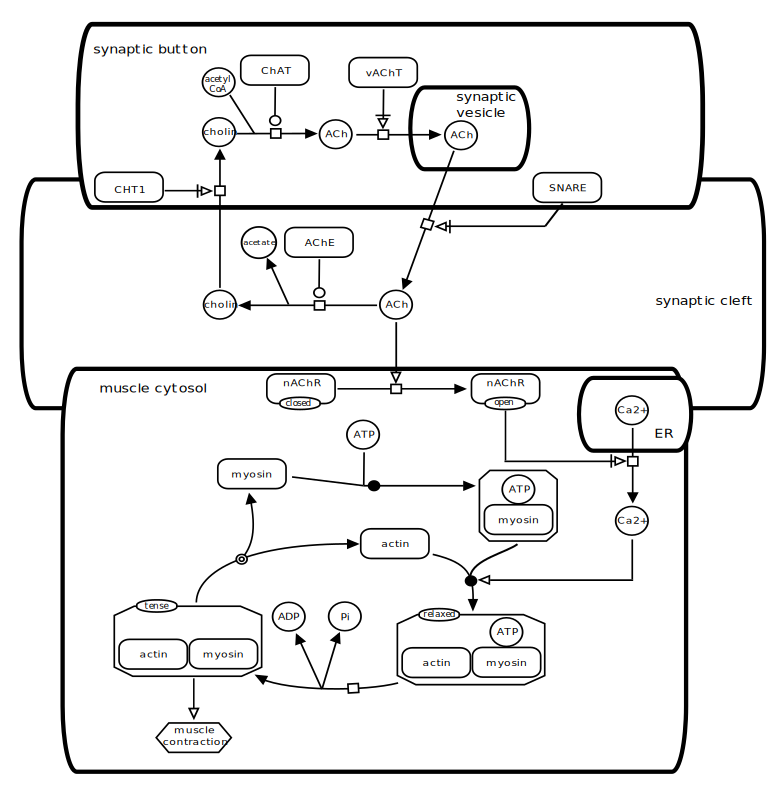
\includegraphics{examples/muscle}}
\caption{Neuronal/Muscle signalling. A description of inter-cellular signalling using SBGN.}\label{fig:muscle}
\end{center}
\end{figure}

\fig{IFN} introduces the use of \SBGNPDLone to encode gene regulatory networks. It also shows the use of the \glyph{empty set} and the \glyph{logical operator} \glyph{and}.

\begin{figure}[htb]
\begin{center}
\scalebox{0.4}{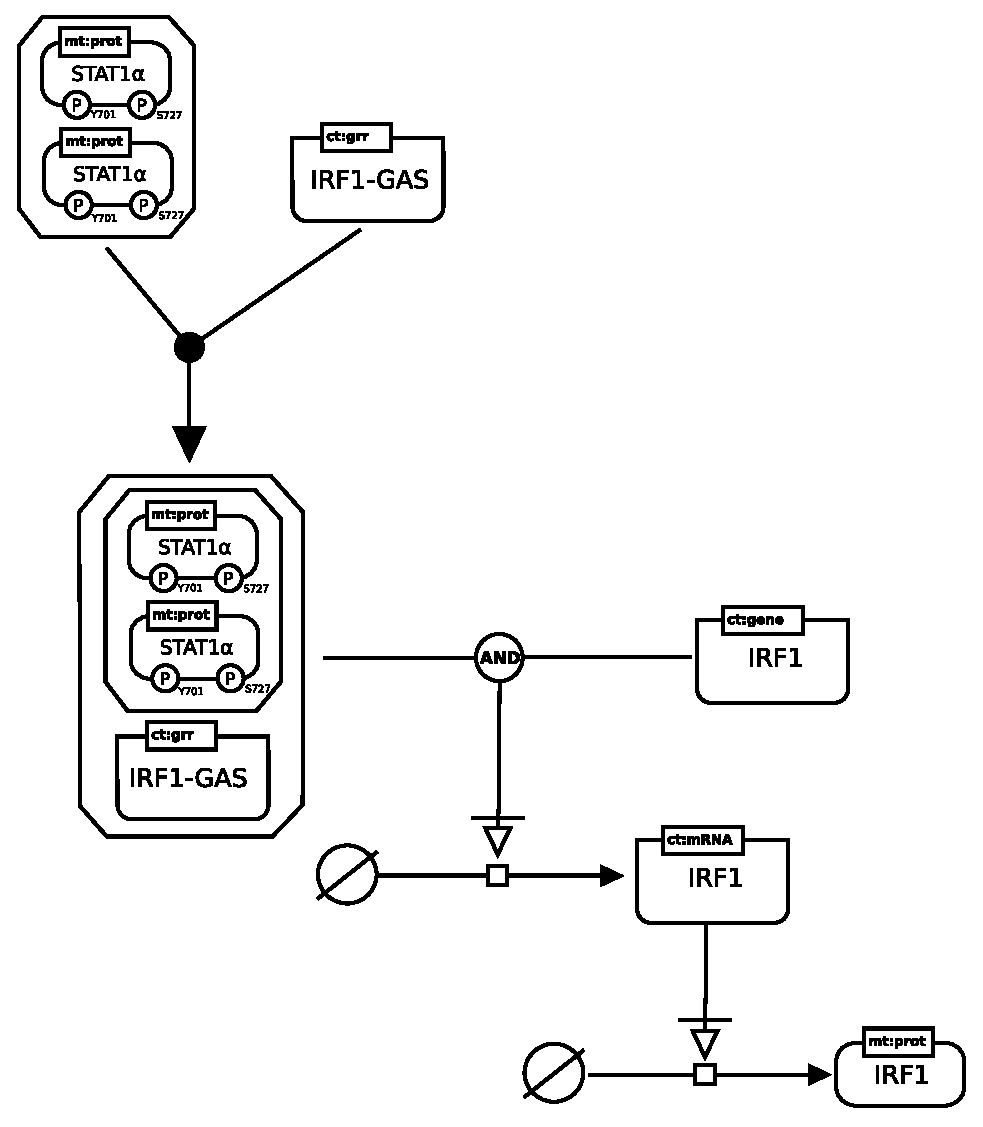
\includegraphics{examples/IFNGeneRef}}
\caption{Activated STAT1$\alpha$ induction of the IRF1 gene. An example of gene regulation using logical operators.}\label{fig:IFN}
\end{center}
\end{figure}
